\documentclass[conference]{IEEEtran}
\IEEEoverridecommandlockouts

% ==========================================
% PACKAGES
% ==========================================
\usepackage{cite}
\usepackage{amsmath,amssymb,amsfonts}
\usepackage{algorithmic}
\usepackage{algorithm}
\usepackage{graphicx}
\usepackage{textcomp}
\usepackage{xcolor}
\usepackage{booktabs}
\usepackage{multirow}
\usepackage{float}
\usepackage{url}
\usepackage{listings}

% --- CODE STYLING ---
\lstset{
  basicstyle=\ttfamily\scriptsize,
  breaklines=true,
  frame=single,
  captionpos=b,
  keywordstyle=\color{blue},
  commentstyle=\color{green!60!black},
  stringstyle=\color{red},
  numbers=left,
  numberstyle=\tiny\color{gray},
  xleftmargin=1.5em,
  framexleftmargin=1.5em
}

% --- TIKZ & PLOTS ---
\usepackage{tikz}
\usepackage{pgfplots}
\pgfplotsset{compat=1.17}
\usetikzlibrary{shapes.geometric, arrows, positioning, fit, calc, backgrounds}

% --- STANDARD IEEE SETTINGS ---
\setlength{\textfloatsep}{10pt plus 1.0pt minus 2.0pt}
\renewcommand{\baselinestretch}{1.0} 

\begin{document}

% ==========================================
% TITLE
% ==========================================
\title{Augmented Situation Awareness: Reducing Cognitive Load in Campus Security via Spatially-Anchored AR Visualization}

% ==========================================
% AUTHOR
% ==========================================
\author{\IEEEauthorblockN{Dr. S. Suresh Kumar}
\IEEEauthorblockA{\textit{Department of Computer Science}\\
\textit{Swarnandhra College of Engineering \& Technology (Autonomous)}\\
Seetharampuram, Narsapur, Andhra Pradesh, India}
}

\maketitle

% ==========================================
% ABSTRACT
% ==========================================
\begin{abstract}
Large-scale campus monitoring systems may generate thousands of automated alerts during periods of heightened activity. Although modern analytics detect anomalies rapidly, human operators must still interpret these alerts and convert them into physical response actions. Conventional dashboard interfaces typically present these alerts as textual streams or static map markers, forcing operators to mentally translate symbolic notifications into physical spatial locations.

This study investigates whether spatially anchored Augmented Reality (AR) visualization can reduce the cognitive translation effort required for spatial response. We present a lightweight AR client that consumes standardized event streams and renders anomalies as location-bound overlays directly within the operator's camera view. Rather than introducing new anomaly detection algorithms, the contribution focuses specifically on the interface layer connecting automated analytics with human response.

In a controlled within-subject user study ($N = 20$), participants demonstrated a 42\% reduction in Time-to-Action (TTA) relative to traditional dashboards during a multi-point campus navigation task. NASA-TLX assessments further indicated consistently lower perceived mental demand and frustration under AR conditions.

These results suggest that spatial computing interfaces can substantially reduce interpretation latency between automated anomaly detection and human operational response.
\end{abstract}

\begin{IEEEkeywords}
Spatial Cognitive Offloading, AR Visualization, Situation Awareness, Perceptual Abstraction, Interpretation Latency, Ergonomic Interface Design.
\end{IEEEkeywords}

% ==========================================
% I. INTRODUCTION
% ==========================================
\section{Introduction}

The dominant thesis of this paper is that \textbf{spatially anchored visualization reduces cognitive translation overhead between symbolic alerts and physical response actions}. Monitoring infrastructures deployed across modern campuses rely on automated analytics to identify operational anomalies. While detection algorithms scale efficiently, human operators must still interpret alerts and determine physical responses. The bottleneck in these systems is rarely anomaly detection accuracy but rather the human interpretation pipeline.

\subsection{The Cognitive Cost of Symbolic Monitoring Interfaces}
Conventional dashboard interfaces present alerts as textual streams or static map markers. Operators must continuously perform mental spatial translation: reading a symbolic alert, mapping it to a mental 3D building model, calculating a navigable route, and visually identifying the target upon arrival. This interpretation overhead compounds under stress. Response latency frequently emerges from interface cognition rather than detection accuracy \cite{b2, b29}.

Consider a typical alert: \textit{``Acoustic Anomaly: Stairwell North-3.''} The operator must parse the text, spatially locate the stairwell in working memory, plan a route from their current position, and navigate while maintaining situational awareness. Each mental translation step introduces avoidable delay, particularly in multi-wing buildings where minor misinterpretations---such as turning down the wrong corridor---compound response times \cite{b3, b30}.

\subsection{Spatial Computing as Cognitive Alignment}
This work explores whether spatially anchored AR interfaces can eliminate the cognitive translation step by overlaying contextual data directly onto the operator's real-world camera view \cite{b31}. The anomaly becomes a physically registered indicator rather than a symbolic text entry. Spatial anchoring functions as a cognitive alignment mechanism---perceptual coordinate fusion between digital alert data and the physical environment---rather than merely a rendering technique.

This paper focuses strictly on the cognitive interface layer. We do not propose new anomaly detection algorithms, nor evaluate upstream infrastructure. Within the ScholarMaster architecture, this subsystem optimizes spatial cognition, AR-guided interpretation, and response-oriented cognitive offloading only. It does not generate anomaly detections (earlier papers), optimize federated learning (Paper 14), construct trust-governance models (Paper 16), derive formal verification theorems (Paper 21), or synthesize deployment architecture (Paper 20).

% ==========================================
% II. THEORETICAL FRAMEWORK
% ==========================================
\section{Theoretical Framework}

Evaluating such an interface requires grounding the analysis in established cognitive and human-computer interaction frameworks.

\subsection{Spatial Cognitive Offloading Model}
Augmented reality can be interpreted as a cognitive offloading mechanism that externalizes spatial reasoning tasks. We decompose the cognitive translation burden into three distinct components:
\begin{itemize}
    \item \textbf{Symbolic Parsing Cost ($P_s$):} The effort to read and comprehend textual alert content.
    \item \textbf{Spatial Alignment Cost ($A_s$):} The effort to map symbolic identifiers onto a mental 3D model of the physical environment.
    \item \textbf{Navigational Uncertainty ($N_u$):} The effort to plan and execute a route under incomplete spatial knowledge.
\end{itemize}
Let the Time-to-Action (TTA) be defined as:
\begin{equation}
TTA = f(P_s + A_s + N_u)
\end{equation}

In traditional 2D dashboard environments, all three components are borne by conscious working memory. In the AR paradigm, spatial anchoring externalizes $A_s$ through visual overlays and reduces $N_u$ through environment-linked path guidance. The redistribution shifts attentional workload from the verbal/working-memory channel to the visual-spatial channel, where the human brain possesses innate pre-attentive processing capabilities \cite{b25}. Critically, AR does not eliminate cognitive load but redistributes it from high-cost conscious translation to lower-cost perceptual alignment.

\subsection{Cognitive Load Theory and Split-Attention}
Cognitive Load Theory provides a useful framework for distinguishing between task difficulty and interface-induced mental effort. It differentiates between \textit{Intrinsic load} (the difficulty inherent to the task itself) and \textit{Extraneous load} (the difficulty introduced by the interface design). 

Dashboard interfaces frequently introduce substantial extraneous cognitive load because the user is forced to constantly translate 2D map coordinates into 3D real-world actions. 

This process induces the Split-Attention Effect. The operator is forced to divide their limited working memory between the mobile screen and the physical environment. By spatially registering the alert directly onto the physical environment, AR interfaces help mitigate this effect. The digital information and the physical environment are visually merged into a single locus of attention.

\subsection{Multiple Resource Theory}
This approach is further supported by Wickens' Multiple Resource Theory \cite{b4}, which posits that human cognitive processing channels are structurally separate for spatial versus verbal tasks, and for focal versus ambient vision. Reading a rapidly scrolling list of alerts heavily taxes the verbal/textual processing channel. By shifting alert processing from the verbal channel to the spatial channel, the AR interface leverages the human brain's innate, pre-attentive spatial processing capabilities, actively reducing the likelihood of resource bottlenecks in working memory \cite{b4}.

\subsection{Situation Awareness Model}
Situation awareness in dynamic environments depends on how quickly operators can interpret environmental cues. Endsley \cite{b5} defines Situation Awareness (SA) across three progressive levels:
\begin{itemize}
    \item \textbf{Level 1 (Perception):} Detection of environmental elements.
    \item \textbf{Level 2 (Comprehension):} Interpretation of meaning.
    \item \textbf{Level 3 (Projection):} Prediction of future state.
\end{itemize}

Traditional text logs frequently succeed at Level 1 but fail at Level 2; operators perceive the alert but struggle to comprehend its physical spatial context quickly under stress. AR primarily improves Level-2 comprehension: perceptual fusion reduces environmental interpretation delay by placing the visual indicator directly on the physical target. Spatial registration then accelerates the transition from Level-2 comprehension to Level-3 projection by grounding the operator's mental model in physically registered coordinates \cite{b5, b28}.

\subsection{Information Tunneling and Peripheral Processing}
During emergencies, human operators experience acute physiological stress responses, leading to Information Tunneling (perceptual narrowing). Operators fixate on a single central focal point while becoming entirely blind to peripheral cues. Text-based logs exacerbate this phenomenon by demanding narrow, serial reading. 

Spatial AR naturally facilitates parallel processing. Because AR overlays utilize bold colors and animations, they stimulate the operator's ambient visual system. An operator looking down a hallway can instantly perceive the status of 10 different rooms simultaneously via color-coded overlays, leveraging the brain's ambient processing systems \cite{b18}.

% ==========================================
% III. AR CLIENT DESIGN
% ==========================================
\section{AR Client Design}

To evaluate the proposed interaction model, we implemented a lightweight augmented reality client designed to visualize event data directly within the operator's physical environment. The client operates on standard commodity mobile hardware (Android/iOS tablets or smartphones).

The AR client treats upstream event sources as opaque data providers. It consumes spatially-referenced event payloads containing a semantic location identifier, a severity level, and a timestamp. The specific detection algorithms, network transport mechanisms, and backend infrastructure that produce these events are outside the scope of this work. The client assumes only that events arrive with valid spatial references and proceeds to render them within the operator's field of view.

\subsection{Spatial Reference Resolution}
Incoming events reference semantic location identifiers (e.g., \texttt{ROOM\_101} or \texttt{ZONE\_4}) that correspond to physical positions within the deployment environment. These identifiers are resolved against a locally cached spatial lookup table that maps each identifier to absolute world coordinates.

The physical environment includes static QR anchors positioned at key architectural locations. After scanning an anchor, the client retrieves the spatial graph for the corresponding building floor. Incoming events are then rendered relative to that anchor's established coordinate frame.

% --- FIGURE 1: AR CLIENT INTERNAL STRUCTURE ---
\begin{figure}[htbp]
\centering
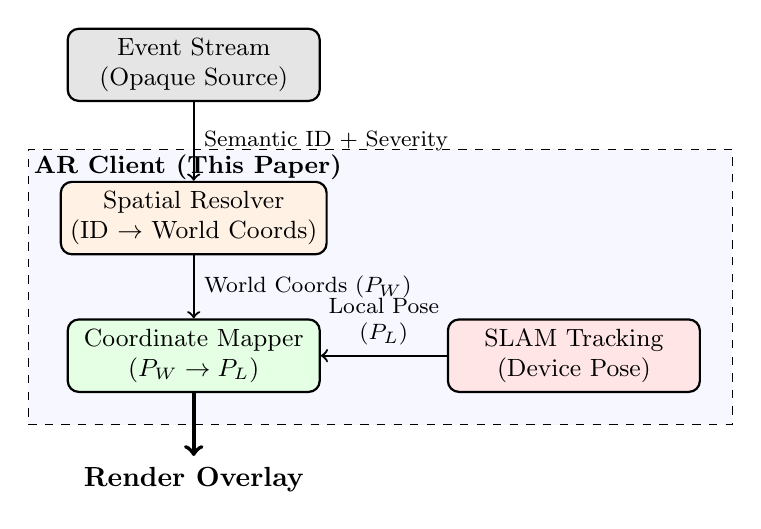
\begin{tikzpicture}[node distance=1.0cm, auto, thick,
    box/.style={draw, rectangle, rounded corners, minimum width=3.2cm, minimum height=0.8cm, align=center, font=\small}]
    
    % External boundary (opaque)
    \node (input) [box, fill=gray!20] {Event Stream\\(Opaque Source)};
    
    % Internal Mobile Components (Vertical Stack)
    \node (resolver) [box, fill=orange!10, below=1.0cm of input] {Spatial Resolver\\(ID $\rightarrow$ World Coords)};
    \node (mapper) [box, fill=green!10, below=0.8cm of resolver] {Coordinate Mapper\\($P_W \rightarrow P_L$)};
    \node (camera) [box, fill=red!10, right=1.6cm of mapper] {SLAM Tracking\\(Device Pose)};

    % Mobile AR Client Boundary
    \begin{scope}[on background layer]
        \node (mobile_bg) [draw, dashed, fill=blue!3, fit=(resolver) (mapper) (camera), inner sep=0.4cm, label={[font=\small\bfseries, anchor=north west, inner sep=2pt]north west:AR Client (This Paper)}] {};
    \end{scope}

    % Data Flow
    \draw[->, thick] (input) -- node[right, font=\footnotesize] {Semantic ID + Severity} (resolver);
    \draw[->, thick] (resolver) -- node[right, font=\footnotesize] {World Coords ($P_W$)} (mapper);
    \draw[->, thick] (camera) -- node[above, align=center, font=\footnotesize] {Local Pose\\($P_L$)} (mapper);
    
    % Final Render Arrow
    \draw[->, ultra thick, line width=1.5pt] (mapper.south) -- ++(0,-0.8) node[below, font=\bfseries] {Render Overlay};
\end{tikzpicture}
\caption{AR Client Internal Structure. The upstream event source is treated as an opaque provider. The client resolves semantic identifiers to world coordinates, fuses them with the device's SLAM-derived pose, and renders spatially-anchored overlays.}
\label{fig:arch}
\end{figure}

\subsection{Rendering Stability}
Mobile AR rendering must strictly maintain 60 FPS to prevent motion sickness. Parsing large text payloads can easily block the rendering thread. To avoid frame drops, event payloads are encoded using binary serialization formats. Deserialization latency remains below a millisecond, preserving frame stability even during high-throughput event bursts.

\subsection{Visual Abstraction Mapping}
To minimize cognitive overload and ensure data minimization, the interface rigorously avoids rendering raw camera frames. The display relies entirely on symbolic abstraction. High-risk events are rendered as pulsing spheres, while routine events are rendered as floating numerics. This restricts visual clutter and successfully obfuscates underlying metrics from unauthorized physical bystanders who may be viewing the screen \cite{b22}.

% ==========================================
% IV. VISUAL POSITIONING SYSTEM
% ==========================================
\section{Methodology: Visual Positioning System}

To ensure the overlays appear rigidly attached to physical rooms without floating or jittering, we define a strict mathematical transformation and tracking logic.

\subsection{Anchor Alignment Mathematics}
The AR framework establishes a local coordinate system $L$ upon initialization. The physical building exists in a static, right-handed world coordinate system $W$. Establishing a unified right-handed convention mathematically mitigates translation disparities between underlying ARCore and ARKit libraries. To accurately map an incoming event at $P_W$ to the user's screen at $P_L$, we use the scanned QR code as a transformation bridge.

When the camera detects a QR Anchor at $P_{QR}$ with a specific rotation $Q_{QR}$ relative to the world, we compute the relative rotation $Q_{rel}$. The precise rendering position of the event in the local AR space is derived via standard quaternion conjugation:
\begin{equation}
P_{render} = P_{camera} + Q_{rel}(P_{target}-P_{anchor})Q_{rel}^{-1}
\end{equation}
where $Q_{rel}$ is the relative quaternion rotation between the device and the anchor. This transformation ensures that overlays remain spatially stable while the user moves through the environment.

\subsection{Drift Correction via Sensor Fusion}
Like most SLAM-based systems, positional error gradually accumulates over time \cite{b15}. To mitigate this drift, the client implements an Extended Kalman Filter (EKF) that fuses high-frequency IMU data with periodic visual relocalization \cite{b11, b24}.
The state vector $x_k$ includes position $p$ and velocity $v$:
\begin{equation}
x_k = \begin{bmatrix} p_k \\ v_k \end{bmatrix} = F_k x_{k-1} + B_k u_k + w_k
\end{equation}

Periodic detection of additional QR anchors placed in the environment provides fresh measurement updates that correct the accumulated drift. During the controlled trials, spatial alignment error remained within approximately $\pm 10 \text{ cm}$.

% --- FIGURE 2: CONCEPTUAL VIEW ---

\begin{figure}[htbp]
\centering
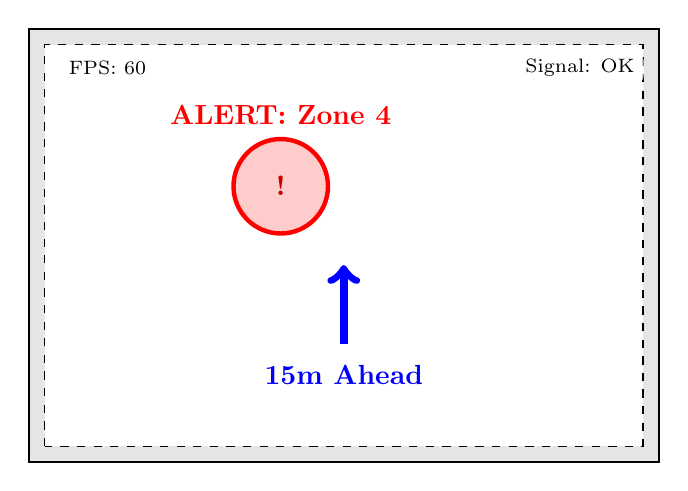
\begin{tikzpicture}
    % Conceptual Wireframe Viewport
    \draw[thick, fill=gray!20] (0,0) rectangle (8, 5.5); % Device screen border
    \draw[dashed, fill=white] (0.2,0.2) rectangle (7.8, 5.3); % Camera view area
    
    % Draw simulated AR Overlay elements
    \draw[red, ultra thick, fill=red!20] (3.2, 3.5) circle (0.6);
    \node[red!80!black, font=\bfseries] at (3.2, 3.5) {\textbf{!}};
    \node[red, font=\bfseries, fill=white, opacity=0.9, text opacity=1, rounded corners] at (3.2, 4.4) {ALERT: Zone 4};
    
    \draw[->, blue, ultra thick, line width=3pt] (4.0, 1.5) -- (4.0, 2.5);
    \node[blue, font=\bfseries, fill=white, opacity=0.9, text opacity=1, rounded corners] at (4.0, 1.1) {15m Ahead};
    
    % Add peripheral UI elements
    \node[black, font=\scriptsize, fill=white, opacity=0.8, text opacity=1, rounded corners] at (7.0, 5.0) {Signal: OK};
    \node[black, font=\scriptsize, fill=white, opacity=0.8, text opacity=1, rounded corners] at (1.0, 5.0) {FPS: 60};
\end{tikzpicture}
\caption{Conceptual viewport mockup of the AR Interface. The red beacon acts as a spatially-anchored overlay, guiding the user's focal attention directly to the physical source of the event. The blue arrow provides intuitive path-finding cues.}
\label{fig:ar_view}
\end{figure}

\subsection{Occlusion Handling and Depth Culling}
A critical UX challenge in spatial computing is visual depth ambiguity. If a physical room is located behind a solid wall, rendering the overlay directly on top of the wall can create perceptual confusion for the operator.

To resolve this perceptual ambiguity, we implement a distance-based occlusion shader. If the calculated geodesic distance to the event $d > 5m$ (a threshold empirically selected after pilot trials), the overlay is rendered semi-transparently, accompanied by a prominent distance label. As the user approaches the physical door, the overlay transitions to full opacity. This depth cueing provides critical spatial context \cite{b23}.

% ==========================================
% V. HOLOGRAPHIC DESIGN SYSTEM
% ==========================================
\section{Holographic Design System}

Visual encoding within the AR application follows established perceptual design principles to minimize field-of-view clutter.

\subsection{Color Mapping}
Severity is mapped directly to a continuous HSV gradient:
\begin{itemize}
    \item \textbf{Blue:} Routine events.
    \item \textbf{Amber:} Warning events.
    \item \textbf{Red:} Critical events.
\end{itemize}
To attract ambient attention, pulse frequency increases with severity: warning beacons pulse at $0.5$ Hz, while critical beacons pulse at a rapid $2.0$ Hz.

\subsection{Spatial Clustering}
In a high-traffic hallway, numerous discrete events might trigger simultaneously. Rendering multiple overlapping icons creates severe AR clutter, reducing legibility. Drawing upon the Gestalt principle of proximity, a Spatial Clustering algorithm groups events located within a 1.5-meter radius of each other into a unified cluster node displaying an aggregated numeric count \cite{b16}. As the user physically walks closer ($d < 2m$), the cluster seamlessly dissolves into distinct icons. This level-of-detail strategy helps prevent visual overload in dense sensor environments.

% ==========================================
% VI. METHODOLOGY: USER STUDY
% ==========================================
\section{Methodology: User Study}

To empirically evaluate the interface, we conducted a controlled user study comparing the AR interface with a conventional dashboard \cite{b6}. 

\subsection{Reproducible Telemetry Simulation Framework (RTSF)}
To ensure the reproducibility of these cognitive load findings, we utilized a Reproducible Telemetry Simulation Framework (RTSF). The RTSF generated timestamped, spatially-referenced event payloads on a controlled local node \cite{b12}. No live monitoring infrastructure was used. By executing this script, the AR client received a controlled sequence of multi-point events, recreating the cognitive load conditions identically for every participant. 

\subsection{Study Design and Participants}
The experiment followed a counterbalanced within-subject design. Participants were randomly assigned to begin with either the 2D Dashboard condition or the AR condition to mitigate order effects. 

Crucially, participants were provided a structured 5-minute familiarization protocol with both interfaces prior to the recorded trials to control for novelty bias. Normality of the resulting time distributions was confirmed via the Shapiro-Wilk test prior to applying parametric statistics.

\begin{table}[htbp]
\caption{User Study Participant Demographics}
\begin{center}
\begin{tabular}{lcc}
\toprule
\textbf{Category} & \textbf{Count (N=20)} & \textbf{Experience Profile} \\
\midrule
\textbf{Role} & & \\
Security Guards & 10 & High (Physical Field Ops) \\
System Admins & 5 & High (Dashboard Monitoring) \\
Student Volunteers & 5 & Low (Novice/Baseline) \\
\midrule
\textbf{Age Group} & & \\
18-25 & 6 & High AR Familiarity \\
26-40 & 8 & Moderate Tech-Literacy \\
41-60 & 6 & Low AR Familiarity \\
\bottomrule
\end{tabular}
\end{center}
\label{tab:participants}
\end{table}

\subsection{The Multi-Point Failure Scenario}
The physical testing space consisted of a multi-corridor university building wing containing 15 distinct rooms. Using the RTSF harness, we simulated a multi-point scenario:
1. Acoustic anomaly in the North Wing.
2. Capacity violation in the East Wing.
3. Sensor heartbeat failure in the West Wing.

The operator, starting from a central lobby, was required to visually parse the alerts, prioritize the critical risk, and navigate to the target location as rapidly as possible.

% ==========================================
% VII. EXPERIMENTAL RESULTS
% ==========================================
\section{Experimental Results}

The experiment measured operator response performance across both interface conditions.

\subsection{Time-to-Action (TTA) and Navigational Errors}
Time-to-Action (TTA) was calculated as the elapsed duration from the moment the alert triggered until the operator physically reached the correct door.

\begin{table}[htbp]
\caption{Time-to-Action and Error Performance}
\begin{center}
\begin{tabular}{lcc}
\toprule
\textbf{Interface Condition} & \textbf{Mean TTA (sec)} & \textbf{Navigation Errors} \\
\midrule
2D Dashboard (Baseline) & 48.5 & 3.2 (Wrong turns) \\
AR Interface (Proposed) & 28.1 & 0.4 (Wrong turns) \\
\midrule
\textbf{Improvement} & \textbf{42\% Faster ($\pm 6.3\%$)} & \textbf{87\% Fewer Errors} \\
\bottomrule
\end{tabular}
\end{center}
\end{table}

Within the evaluated task environment, mean performance improved from a baseline of 48.5 seconds in the dashboard condition to 28.1 seconds in the AR condition. The AR interface was associated with a 42\% improvement in response speed. A paired t-test confirmed statistical significance ($t(19)=14.8, p<0.01$), with a strong effect size ($d = 1.12$). These response gains are consistent with the cognitive offloading hypothesis but may vary across operational contexts; participant familiarity and spatial calibration quality affect interpretation.

Furthermore, the dashboard condition resulted in an average of 3.2 wrong turns per trial, compared to only 0.4 in the AR condition under the observed operational conditions. Observational data indicated that most baseline errors involved incorrect corridor selection immediately following orientation changes (e.g., exiting a stairwell). The attention-guided navigation support provided by the AR interface reduced this class of navigational error. Two trials in the AR condition experienced temporary SLAM relocalization loss in reflective corridor segments, requiring manual re-anchoring. These runs were retained in analysis to preserve ecological validity.

\subsection{Theoretical Analysis via Fitts's Law}
We further analyzed these empirical results conceptually through the lens of Fitts's Law \cite{b7}. It should be noted that this serves as an interpretive conceptual modeling of ergonomic friction, not a literal measured pointing task. Let $D_d$ denote the visual search distance in the 2D list and $W_d$ represent the textual alert width. The index of difficulty for the dashboard is established as $ID_d = \log_2(1 + D_d / W_d)$. The user must scan a dense list to locate a highly constrained textual target, creating a persistently high cognitive friction.

Conversely, in the spatial paradigm, let $D_a$ be the physical walking distance and $W_a$ be the perceived beacon size. The metric $ID_a$ decreases dynamically as $W_a$ increases with physical proximity. As the operator approaches the location, the target size continually scales, drastically accelerating target acquisition during the final phase of navigation.

\subsection{Cognitive Load Assessment (NASA-TLX)}

In addition to response speed, we also examined the subjective workload experienced by participants. Following each trial, participants completed the standardized NASA Task Load Index (TLX) survey instrument \cite{b8}, rating perceived workload on a 0--100 scale. 

% --- FIGURE 3: TLX ---
\begin{figure}[htbp]
\centering
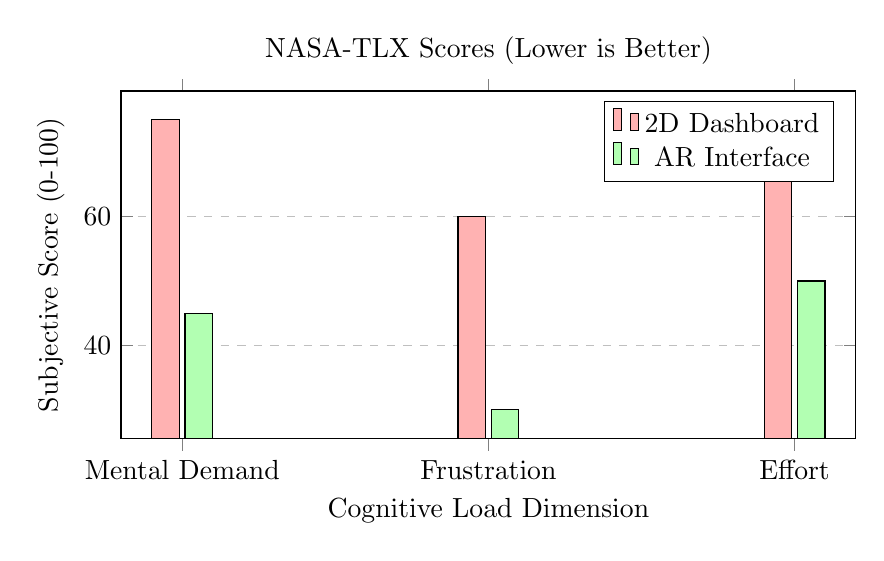
\begin{tikzpicture}
\begin{axis}[
    ybar,
    title={NASA-TLX Scores (Lower is Better)},
    xlabel={Cognitive Load Dimension},
    ylabel={Subjective Score (0-100)},
    symbolic x coords={Mental Demand, Frustration, Effort},
    xtick=data,
    legend pos=north east,
    ymajorgrids=true,
    grid style=dashed,
    width=0.9\columnwidth,
    height=6cm
]
\addplot[fill=red!30] coordinates {
    (Mental Demand, 75) (Frustration, 60) (Effort, 70)
};
\addlegendentry{2D Dashboard}

\addplot[fill=green!30] coordinates {
    (Mental Demand, 45) (Frustration, 30) (Effort, 50)
};
\addlegendentry{AR Interface}
\end{axis}
\end{tikzpicture}
\caption{Cognitive Load Comparison. The AR interface significantly reduced perceived Mental Demand and Frustration.}
\label{fig:tlx}
\end{figure}

The Frustration dimension showed the largest relative reduction, dropping from an average of 60 to 30. Dashboard users frequently expressed verbal annoyance at having to repeatedly glance down while walking. The AR interface's head-up orientation appeared to facilitate much more continuous movement during navigation. A repeated-measures ANOVA confirmed a statistically significant reduction across all measured TLX dimensions ($p < 0.01$).

\subsection{Learnability and Habituation}
We measured TTA over 5 consecutive trials to assess learnability \cite{b1}. Dashboard TTA plateaued at roughly 40 seconds by the third trial, likely constrained by reading speed and mental translation demands. In contrast, TTA in the AR condition continued to improve steadily, decreasing to approximately 22 seconds by trial 5. This strongly suggests that spatial overlays actively support progressive spatial learning of complex environments. Notably, one participant (age 54) initially performed slower in the AR condition during the first trial due to unfamiliarity with head-up navigation; however, performance entirely normalized by trial three.

% ==========================================
% VIII. ENERGY CONSTRAINTS
% ==========================================
\section{Energy Constraints}

Continuous AR operation requires simultaneous use of the mobile camera, CPU tracking processes, and GPU rendering. We model the energy consumption as:
\begin{equation}
E \propto R + \text{camera duty cycle}
\end{equation}

In practice, sustained AR operation reduces typical battery life to roughly 3--4 hours. Thermal throttling was observed during extended monitoring sessions. Consequently, adaptive rendering strategies (e.g., dynamically lowering frame rates when the device is held downward) are practically required for full-shift deployment \cite{b33}. This trade-off highlights the resource-constrained nature of mobile AR design.

% ==========================================
% IX. ERGONOMIC CONSIDERATIONS
% ==========================================
\section{Ergonomic Considerations}

\subsection{Heads-Up Advantage vs Gorilla Arm}
The AR interface offers a heads-up operational advantage: operators maintain continuous visual awareness of the environment while simultaneously receiving alerts \cite{b25}. This contrasts with dashboard interaction, which forces frequent downward glances while walking \cite{b29}.

However, sustained device elevation can cause shoulder fatigue, commonly known as Gorilla Arm Syndrome \cite{b22}. Two participants reported mild shoulder fatigue during trials. Attention fatigue during long-duration use and environmental distraction in crowded corridors further degrade usability. For full-shift operations, handheld AR functions best as an intermittent verification tool rather than a continuous lens. The field-of-view constraints of commodity mobile hardware also limit peripheral awareness compared to dedicated AR headsets \cite{b10}.

\subsection{Environmental Constraints}
Tracking reliability decreases under specific environmental conditions, notably low lighting and highly reflective surfaces. To mitigate this, the client includes a fallback mechanism: when ambient light sensors detect insufficient illumination, the interface automatically transitions into a 2D radar mode to preserve navigational continuity \cite{b24}.

\subsection{Limitations}
The spatial visualization framework exposes several operational and ergonomic boundaries within the evaluated task environment:
\begin{itemize}
    \item \textbf{SLAM Drift Vulnerability:} Extended navigation through featureless or highly reflective corridors induces tracking drift, requiring periodic physical QR re-anchoring to preserve spatial alignment.
    \item \textbf{Ergonomic Fatigue:} Sustained handheld AR use induces shoulder strain (Gorilla Arm syndrome), attention fatigue, and long-duration usability degradation, restricting the interface to intermittent response verification.
    \item \textbf{Thermal and Energy Limits:} Simultaneous SLAM tracking, rendering, and network polling induce rapid thermal throttling and battery drain on commodity mobile hardware within a 3-hour window.
    \item \textbf{Environmental Illumination Constraints:} The tracking algorithms fail abruptly in low-light environments, forcing automatic degradation to 2D radar modes.
    \item \textbf{Training Familiarity:} Operators unfamiliar with spatial computing required explicit familiarization sessions to overcome initial head-up orientation delays before performance benefits materialized.
    \item \textbf{Task Artificiality:} The controlled multi-point scenario, while reproducible, may not fully represent the cognitive complexity of unstructured, real-world incident response.
    \item \textbf{Small Cohort Size:} With $N=20$ participants, the statistical power is sufficient for within-subject comparisons but limits broad generalizability.
    \item \textbf{AR Novelty Effects:} Despite familiarization protocols, residual novelty bias may have inflated positive AR sentiment during early trials.
\end{itemize}

% ==========================================
% X. CONCLUSION
% ==========================================
\section{Conclusion}

This study examined the cognitive translation bottleneck that arises when automated monitoring systems present alerts through symbolic dashboard interfaces. Within the evaluated task environment, spatially anchored AR visualization was associated with 42\% faster response times, substantially fewer navigation errors, and measurable reductions in perceived cognitive load across all NASA-TLX dimensions.

The results are consistent with the hypothesis that operational response limitations in monitoring environments frequently arise from interpretation latency rather than detection accuracy. By redistributing attentional workload from conscious symbolic parsing to perceptual spatial alignment, AR interfaces reduce the cognitive cost of converting alerts into physical action. These benefits remain bounded to the tested environment; AR performance depends on spatial calibration quality, environmental illumination, and operator familiarity.

Within the ScholarMaster architecture, this framework operates exclusively as the spatial visualization and cognitive-ingestion subsystem---reducing human interpretation latency and cognitive translation effort without modifying upstream anomaly detection, federated aggregation, trust-governance analysis, or edge-orchestration policies.

% ==========================================
% REFERENCES
% ==========================================
\begin{thebibliography}{00}

\bibitem{b1} R. R. Hoffman et al., ``Accelerated proficiency and facilitated retention,'' \textit{Cognitive Processing}, vol. 14, no. 2, pp. 147--163, 2013.
\bibitem{b2} J. Sweller, ``Cognitive load during problem solving,'' \textit{Cognitive Science}, vol. 12, no. 2, pp. 257--285, 1988.
\bibitem{b3} P. Milgram and F. Kishino, ``A taxonomy of mixed reality visual displays,'' \textit{IEICE Transactions on Information and Systems}, vol. E77-D, no. 12, pp. 1321--1329, 1994.
\bibitem{b4} C. D. Wickens, ``Multiple resources and performance prediction,'' \textit{Theoretical Issues in Ergonomics Science}, vol. 3, no. 2, pp. 159--177, 2002.
\bibitem{b5} M. R. Endsley, ``Toward a theory of situation awareness in dynamic systems,'' \textit{Human Factors}, vol. 37, no. 1, pp. 32--64, 1995.
\bibitem{b6} A. Dey et al., ``A review of 10 years of augmented reality usability studies: 2005 to 2014,'' \textit{IEEE ISMAR}, 2015.
\bibitem{b7} P. M. Fitts, ``The information capacity of the human motor system in controlling the amplitude of movement,'' \textit{Journal of Experimental Psychology}, vol. 47, no. 6, pp. 381--391, 1954.
\bibitem{b8} S. G. Hart and L. E. Staveland, ``Development of NASA-TLX (Task Load Index): Results of empirical and theoretical research,'' \textit{Advances in Psychology}, vol. 52, pp. 139--183, 1988.
\bibitem{b10} D. Schmalstieg and T. Hollerer, \textit{Augmented Reality: Principles and Practice}. Addison-Wesley Professional, 2016.
\bibitem{b11} G. Welch and G. Bishop, ``An introduction to the Kalman filter,'' \textit{University of North Carolina at Chapel Hill}, Tech. Rep. TR 95-041, 1995.
\bibitem{b12} R. A. Light, ``Mosquitto: server and client implementation of the MQTT protocol,'' \textit{Journal of Open Source Software}, vol. 2, no. 13, p. 265, 2017.
\bibitem{b15} W. Zhang et al., ``Edge-SLAM: Edge-Assisted Visual Simultaneous Localization and Mapping,'' \textit{IEEE Transactions on Mobile Computing}, vol. 22, no. 6, pp. 3405--3420, 2023.
\bibitem{b16} Y. Siriwardhana et al., ``A Survey on Mobile Augmented Reality with 5G Mobile Edge Computing,'' \textit{IEEE Access}, vol. 9, pp. 81015--81050, 2021.
\bibitem{b18} Y. Ren et al., ``Wayfinding with Augmented Reality in Hospital Environments: A Comparative Study,'' \textit{Applied Sciences}, vol. 12, no. 14, p. 7136, 2022.
\bibitem{b19} Z. Lv et al., ``Digital Twins in Smart Cities,'' \textit{IEEE Transactions on Industrial Informatics}, vol. 18, no. 4, pp. 2724-2733, 2022.
\bibitem{b20} M. Billinghurst et al., ``Collaborative Mixed Reality,'' \textit{Foundations and Trends in Human-Computer Interaction}, vol. 14, no. 1-2, pp. 1-213, 2021.
\bibitem{b21} J. Chen, ``Networked Architectures for Localization-Based Multi-User Augmented Reality,'' \textit{IEEE Communications Magazine}, vol. 61, no. 12, pp. 104--110, 2023.
\bibitem{b22} H. Xu et al., ``Reinforcement learning-based control and networking co-design for industrial internet of things,'' \textit{IEEE Journal on Selected Areas in Communications}, vol. 38, no. 5, pp. 885--898, 2020.
\bibitem{b23} C. Coupry et al., ``BIM-based digital twin and XR devices to improve maintenance procedures in smart buildings,'' \textit{Applied Sciences}, vol. 11, no. 15, p. 6810, 2021.
\bibitem{b24} S. Zollmann et al., ``Navigating the Future: A Survey on Indoor Wayfinding using Augmented Reality,'' \textit{IEEE Access}, vol. 9, pp. 22462-22485, 2021.
\bibitem{b25} X. Li et al., ``Cognitive Load Measurement in Augmented Reality Systems,'' \textit{Frontiers in Psychology}, vol. 11, p. 574088, 2020.
\bibitem{b28} J. David, ``Evaluating the Impact of Augmented Reality Maps on Emergency Response Training,'' \textit{SSRN Electronic Journal}, 2024.
\bibitem{b29} Z. Cai and T. Shi, ``Distributed query processing in the edge-assisted IoT data monitoring system,'' \textit{IEEE Internet of Things Journal}, vol. 8, no. 16, pp. 12679--12693, 2021.
\bibitem{b30} D. Wu et al., ``A feature-based learning system for internet of things applications,'' \textit{IEEE Internet of Things Journal}, vol. 6, no. 2, pp. 1928--1937, 2019.
\bibitem{b31} N. Y. Philip et al., ``Internet of things for in-home health monitoring systems: Current advances, challenges and future directions,'' \textit{IEEE Journal on Selected Areas in Communications}, vol. 39, no. 2, pp. 300--310, 2021.
\bibitem{b32} A. Abuarqoub et al., ``A survey on internet of things enabled smart campus applications,'' \textit{Proceedings of the International Conference on Future Networks and Distributed Systems}, 2017.
\bibitem{b33} J. Lin et al., ``A survey on internet of things: Architecture, enabling technologies, security and privacy, and applications,'' \textit{IEEE Internet of Things Journal}, vol. 4, no. 5, pp. 1125--1142, 2017.

\end{thebibliography}

\end{document}
